\documentclass[monografia]{subfiles}

\begin{document}

	\chapter{Fundamentação Teórica}	
		Neste capítulo está a base teórica, de forma resumida, das operações matemáticas efetuadas neste trabalho para o processamentos do áudios. 
		Na Seção \ref{sec:fourierTransform} é apresentada a transformada de \textit{Fourier}, assim como sua importância na área de processamento
		de sinais. A transformada discreta de \textit{Fourier} é apresentada na Seção \ref{sec:digitalFourierTransform}, esta 
		que é uma versão discretizada da transformada de \textit{Fourier}. Na última seção deste capítulo, \ref{sec:goertzelAlgorithm}, apresentamos o 
		algoritmo de \textit{Goertzel}, que é uma versão derivada da transformada discreta de \textit{Fourier}. É com o uso do algoritmo
		de \textit{Goertzel} que são efetuados
		os processamentos de sinais deste trabalho. As seções abordadas neste capítulo, tiveram como fonte de estudo \cite{oppenheim}.

	\section{Transformada de Fourier}
	\label{sec:fourierTransform}
		A transformada de \textit{Fourier} é uma operação matemática de fundamental importância no campo de processamento de sinais.
		Em essência, este operador faz a transição de funções que têm se comportamento descrito no tempo, para o domínio da
		frequência, com o caminho inverso também sendo possível, permitindo a análise das componentes de frequência do sinal.

		A transformada de \textit{Fourier} tem sua origem na série de \textit{Fourier}, que é uma forma de representação de funções periódicas 
		através da combinação linear de funções trigonométricas. A equação \ref{eq:fourieSerie} representa a série de \textit{Fourier}.
		Os valores do parâmetros da série são encontrados usando as relações apresentadas em \ref{eq:fourieSerieCoeffs}.

			\begin{align}
			\label{eq:fourieSerie}
				&f(t)  = a_{0} + \sum_{n=1}^{\infty }[a_{n} cos(n \omega_{0} t) + b_{n} sen(n \omega_{0} t)] 
			\end{align}


			\begin{align}
			\label{eq:fourieSerieCoeffs}
				&a_{0} = \frac{1}{T} \int_{t_{0}}^{t_{0}+T}f(t)dt \\
				&a_{n} = \frac{2}{T} \int_{t_{0}}^{t_{0}+T}f(t) cos(n \omega_{0} t)dt \\
				&b_{n} = \frac{2}{T} \int_{t_{0}}^{t_{0}+T}f(t) sen(n \omega_{0} t)dt				
			\end{align}

		Representado a série de \textit{Fourier} na forma exponencial, temos:

			\begin{align}
			\label{eq:fourieSerie}
				f(t) & = \sum_{n=-\infty}^{\infty}C_{n} e^{j n \omega_{0} t} \textrm{, tendo o valor de } c_{n} \textrm{obtido de:}\\
				% C_{n} &= \frac{1}{T} \int_{  -\frac{T}{2}   }^{\frac{T}{2}}f(t) e^{-j n \omega_{0} t}dt
			\end{align}

			\begin{align}
			\label{eq:fourieSerieC}
				C_{n} &= \frac{1}{T} \int_{  -\frac{T}{2}   }^{\frac{T}{2}}f(t) e^{-j n \omega_{0} t}dt
			\end{align}

			Para um caso limite da série de \textit{Fourier}, fazendo $T \rightarrow \infty$, o que significa dizer que a função é aperiódica, a distância
			entre as harmônicas $n\omega_{0}$ e $(n+1)\omega_{0}$ torna-se cada vez menor. Matematicamente temos:

			\begin{align}
				& \Delta \omega = (n+1)\omega_{0} - n\omega_{0} = \omega_{0} = \frac{2\pi}{T} \Rightarrow 
				\frac{1}{T} = \frac{\Delta \omega}{2 \pi}\\
				\textrm{Fazendo } & T \rightarrow \infty \Rightarrow \frac{1}{T} \rightarrow  \frac{d\omega}{2 \pi} 
			\end{align}

			Portando, fazer $T \rightarrow \infty \Rightarrow n\omega_{0}\rightarrow \omega$,
			ou seja, frequência deixa de ser uma variável discreta e passa a ser uma variável contínua. Portando a partir de \ref{eq:fourieSerie}, 
			tendo que $T \rightarrow \infty$, temos:

			\begin{align}
				\label{eq:fourierTrans}
				&C_{n}T \rightarrow \int_{-\infty}^{\infty}f(t)e^{-j \omega t}dt \\
				&F(\omega) = \int_{-\infty}^{\infty}f(t)e^{-j \omega t}dt  
			\end{align}

				A integral presente na equação \ref{eq:fourierTrans} é conhecida como a transformada de \textit{Fourier}. A transformada inversa de \textit{Fourier}
				é obtida através de \ref{eq:fourieSerie}, fazendo $T \rightarrow \infty$, como é mostrado a seguir:

			\begin{align}
				&f(t) = \frac{T}{T} \sum_{n=-\infty}^{\infty}C_{n} e^{j n \omega_{0} t} = \sum_{n=-\infty}^{\infty}(C_{n}T) e^{j n \omega_{0} t} \frac{1}{T}\\
			\end{align}
				
			Com $T \rightarrow \infty$ , temos que o somatório torna-se uma integral e que:
							
			\begin{align}
				&C_{n}T\rightarrow F(\omega)\\
				&\frac{1}{T} \rightarrow \frac{d\omega}{2\pi} \\
				&f(t) = \frac{1}{2\pi} \int_{-\infty}^{\infty}F(\omega)e^{j \omega t}d\omega
			\end{align}

		\newpage

	\section{Transformada Discreta de Fourier}
	\label{sec:digitalFourierTransform}
		Veremos nessa seção que a transformada discreta de \textit{Fourier} (DFT) é uma versão discretizada da transformada de \textit{Fourier}, 
		e que o resultado do cálculo dos coeficientes da DFT fornece uma aproximação para seus respectivos coeficientes da série de \textit{Fourier}.

		Considerando uma sequência periódica $x[n]$, com período N, tal que $x[n] = x[n+rN]$, com $r,n \in {Inteiros}$. Temos que a representação
		de $x[n]$ pela série de \textit{Fourier}  é dada por $x[n] = \sum_{k=0}^{N-1}X[k] e^{j \frac{2\pi}{N} kn}$, 
		com o cálculo dos coeficientes dado por $X[k] = \sum_{n=0}^{N-1}x[n] e^{-j \frac{2\pi}{N} kn}$. Fazendo $W_{N}=e^{-j \frac{2\pi}{N} }$, temos:

		\begin{align}
			\textrm{Equação de análise}: &x[n] = \sum_{k=0}^{N-1}X[k] W_{N}^{kn} \\
			\textrm{Equação de síntese}: &X[k] = \sum_{n=0}^{N-1}x[n] W_{N}^{-kn}
		\end{align}

		Que é a representação da série discreta de \textit{Fourier} (DFS). Do cálculo dos coeficientes da DFS, temos que:

		 \begin{equation}
		 \label{eq:DFT1}
				X[k] = \left\{\begin{array}{rc}
				\sum_{n=0}^{N-1}x[n] W_{N}^{kn},& 0 \le k \le N-1,\\
				0																			,& \textit{Caso contrário}
			\end{array}\right.
			\end{equation}

			\begin{equation}
				x[n] = \left\{\begin{array}{rc}
				\sum_{k=0}^{N-1}X[k] W_{N}^{-kn},& 0 \le k \le N-1,\\
				0																			,& \textit{Caso contrário}
			\end{array}\right.
			\end{equation}

		O equação \ref{eq:DFT1} diz respeito a cálculo da transformada discreta de \textit{Fourier}


		
	\section{Algoritmo de Goertzel}
	\label{sec:goertzelAlgorithm}
    O algoritmo de \textit{Goertzel} é uma derivação direta da transformada discreta de \textit{Fourier}, usado para reduzir o tempo de computação,
    portanto, diminuir o custo computacional do cálculo dos coeficientes da DFT. Tem seu uso indicado para casos em que é necessário calcular apenas
    alguns pontos do espectro de frequência. 
    O algoritmo de Goertzel é amplamente utilizado na área de processamento de sinais, em \cite{Zaplata} é apresentado este algoritmo sendo usado como
    um filtro. \cite{Selman} mostra uma comparação, que inclui o algoritmo de Goertzel, mostrando seu desempenho em relação à outra técnicas na detecção DTMF.
    \cite{Yuying}, em seu trabalho, fala sobre a utilização do algoritmo de Goertzel na detecção de tons DTMF, assim como sua implementação em \textit{MATLAB}.
    
    Na Seção \ref{sec:digitalFourierTransform}, definimos $W_{N}=e^{-j \frac{2\pi}{N}}$, fazendo $n=N$, 
    temos:

		\begin{align}
	    W_{N}^{-kN} = e^{j \frac{2\pi}{N}kN} = e^{j 2\pi k} = 1
		\end{align}

		Portanto temos a partir da equação \ref{eq:DFT1}:

		\begin{align}
			X[k] = \sum_{r=0}^{N-1}x[n] W_{N}^{kr} = W_{N}^{-kN} \sum_{n=0}^{N-1}x[n] W_{n}^{kr} = \sum_{n=0}^{N-1}x[n] W_{n}^{-k(N-r)}
		\end{align}

		Definindo a função de resposta ao impulso temos:

		\begin{align}
			&h_{k}[n] = W_{N}^{-kn} u[n] = e^{j \frac{2 \pi}{N} kn} u[n]%\textrm{, com a resposta ao impulso temos como calcular a saída:}\\
			% &y_{k}[n] = x[n] * h_{k}[n]
		\end{align}

		Com a resposta ao impulso temos como calcular a saída:

		\begin{align}
			&y_{k}[n] = x[n] * h_{k}[n]
		\end{align}


		Podemos notar que:

		\begin{align}
			y_{k}[n]	&= \sum_{r=-\infty}^{\infty} x[r]h_k[n-r]\\
								&= \sum_{r=0}^{\infty}x[r]  W_{N}^{-k(n-r)} u[n-r] \textit{, pois } x[r] = 0 \textit{, para } r<0\\
								&= \sum_{r=0}^{n}x[r]  W_{N}^{-k(n-r)} \textit{, pois } u[n-r] = 0 \textit{, para } r>n
		\end{align}

		O valor de $y_k[n]$ para $n=N$ é:

		\begin{align}
			y_{k}[N]	&= \sum_{r=0}^{N}x[r]  W_{N}^{-k(N-r)}\\
								&= \sum_{r=0}^{N-1}x[r]  W_{N}^{-k(N-r)}\textit{, ou seja}\\
								&X[k] = y_k[n]|_{n=N}
		\end{align}

		Portanto podemos interpretar que a DFT de uma sequência $x[n]$ é a saída de um sistema linear invariante no tempo, com a resposta
		impulsiva $W_N^{-kn}u[n]$, calculada no instante $n=N$. 
		
		Da resposta ao impulso, $h_k[n]$, temos que a função de transferência do sistema é:

		\begin{align}
			H_k(z) = \frac{1}{1 - W_N^{-k} z^{-1}}
		\end{align}

		E a equação de diferenças:

		\begin{align}
			y_k[n] = x[n] + W_N^{-k} y_k[n-1], \textit{ com } y_k[-1]=0
		\end{align}

		Para cada $y_k[n]$ calculado, são executadas 4 multiplicações reais, ou 1 complexa. Como deve ser calculado até $n=N$, têm-se
		$N$ multiplicações complexas e $4N$ multiplicações reais.

		A partir da expressão de $H_k(z)$, temos:

		\begin{align}
			H_k(z)	&= H_k(z) \frac{1 - W_N^{-k} z^{-1}}{1 - W_N^{-k} z^{-1}}\\
							&= \frac{1 - W_N^{-k} z^{-1}}{(1 - W_N^{-k} z^{-1})(1 - W_N^{-k} z^{-1})}\\
							&= \frac{1 - W_N^{-k} z^{-1}}{1 - 2\cos(\frac{2 \pi k}{N}) z^{-1} + z^{-2}  }\\
							&= {\left ( \frac{1}{1 - 2\cos(\frac{2 \pi k}{N}) z^{-1} + z^{-2}} \right )} {\left ( 1 - W_N^{-k} z^{-1} \right )}
		\end{align}

		% ( 1 - W_N^{-k} z^{-1}

		O sistema $H_k(z)$ pode ser implementado através da seguinte forma:

		\begin{figure}[!h]
		\centering 
			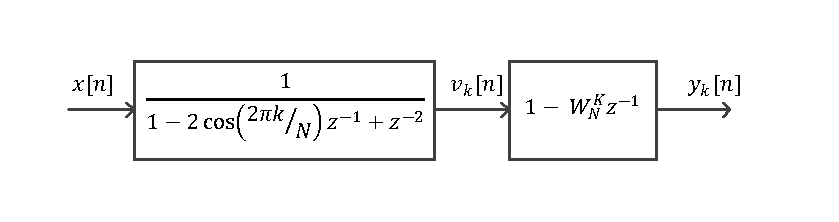
\includegraphics[scale=1.1]{img/HK_systemBlock.pdf}
		% \caption{}
		\label{fig:systemHKBlock}
		\end{figure}

		Temos que:

			\begin{align}
			& v_k[n] = x[n] + 2 \cos(\frac{2 \pi k}{N}) v_k[n-1] - v_k[n-2], v_k[-1] = v_k[-2] = 0 , \textit{ e}\\  
			& y_k[n] = v_k[n] - W_N^{k} v_k[n-1]										
		\end{align}

		Temos que o sinal $v_k[n]$ é calculado para o intervalo $0 \le n \le N$, e o sinal $y_k[n]$ só precisa ser calculado para $n=N$. Para 
		o cálculo do algoritmo, também é preciso armazenar os coeficientes $\cos(\frac{2 \pi k}{N})$ e $W_N^{k}$ para cada k.	

\end{document}
